%%%%%%%%%%%%%%%%%%%%%%%%%%%%%%%%%%%%%%%%%%%%%%%%%%%%%%%%%%%%%%%%%%%%%%
% amspaper.tex --  LaTeX2e-based template for submissions to American 
% Meteorological Society Journals, including
%
% JAS 	-- Journal of the Atmospheric Sciences
% JAMC 	-- Journal of Applied Meteorology and Climatology
% JPO 	-- Journal of Physical Oceanography
% MWR 	-- Monthly Weather Review
% JTECH -- Journal of Atmospheric and Oceanic Technology
% WAF 	-- Weather and Forecasting
% JCLI 	-- Journal of Climate
% JHM 	-- Journal of Hydrometeorology
% JAM 	-- Journal of Applied Meteorology
%
% Template developed by B. Papa and S. Cooley, AMS. 
% Email questions to latex@ametsoc.org.
%
% August 12, 2008 (SRC)
%	- Clarified/added header notes, comments throughout
%	- Improved title page
%	- Edited text of document for clarity
%	- Altered list styles to adhere to AMS style, added comments
%	- Removed incorrect commands (i.e., \catcode) (corrects umlaut bug)
%	- Moved non-template commands to ametsoc.sty
%
% August, 2008 - B. Papa
% - Updated to handle two column journal page output
% - Updated text with new/modified instructions
%
%%%%%%%%%%%%%%%%%%%%%%%%%%%%%%%%%%%%%%%%%%%%%%%%%%%%%%%%%%%%%%%%     
%%%%%%%%%%%%%%%%%%%%%%%%%%%%%%%%%%%%%%%%%%%%%%%%%%%%%%%%%%%%%%%%
%																															 %
%				USE THIS TEMPLATE, AMETSOC.STY, AND AMETSOC.BST				 %
%			        OR YOUR TEX FILES WILL NOT BE USED				  		 %
%																															 % 
%%%%%%%%%%%%%%%%%%%%%%%%%%%%%%%%%%%%%%%%%%%%%%%%%%%%%%%%%%%%%%%%
%%%%%%%%%%%%%%%%%%%%%%%%%%%%%%%%%%%%%%%%%%%%%%%%%%%%%%%%%%%%%%%%

%%%%%%%%%%%%%%%%%%%%%%%%%%%%%%%%%%%%%%%%%%%%%%%%%%%%%%%%%%%%%%%%%%%%%
% PREAMBLE
%%%%%%%%%%%%%%%%%%%%%%%%%%%%%%%%%%%%%%%%%%%%%%%%%%%%%%%%%%%%%%%%%%%%%
%
% The following two commands will generate a PDF that follows all the requirements for submission
% and peer review.  Uncomment these commands to generate this output (and comment out the two lines below.)
%
% DOUBLE SPACE VERSION FOR SUBMISSION TO THE AMS
\documentclass[12pt]{article}
\usepackage{ametsoc}
%
% The following two commands will generate a single space, double column paper that closely
% matches an AMS journal page.  Uncomment these commands to generate this output (and comment
% out the two lines above. FOR AUTHOR USE ONLY. PAPERS SUBMITTED IN THIS FORMAT WILL BE RETURNED
% TO THE AUTHOR for submission with the correct formatting.
%
% TWO COLUMN JOURNAL PAGE LAYOUT FOR AUTHOR USE ONLY
%%%\documentclass[10pt]{article}
%%%\usepackage{ametsoc2col}
%
%%%%%%%%%%%%%%%%%%%%%%%%%%%%%%%%%%%%%%%%%%%%%%%%%%%%%%%%%%%%%%%%%%%%%
% ABSTRACT
%
% Enter your Abstract here
%%%%%%%%%%%%%%%%%%%%%%%%%%%%%%%%%%%%%%%%%%%%%%%%%%%%%%%%%%%%%%%%%%%%%
\newcommand{\myabstract}{Enter the text of your abstract here. This is a sample American Meteorological Society (AMS) \LaTeX\ template.   This document provides authors with both a \LaTeX\ template and basic AMS formatting guidelines to be used when writing a paper.  Authors should refer to the file amspaper.tex to review the actual \LaTeX\ code used to create this document. The amspaper.tex (or blank\_template.tex) file can then be modified by authors for their own manuscript. The abstract should be no longer than 250 words in length.  The abstract should not contain any mathematical expressions, should include no
footnotes or citations, and should not contain first-person sentence structure.}
%
\begin{document}
%
%%%%%%%%%%%%%%%%%%%%%%%%%%%%%%%%%%%%%%%%%%%%%%%%%%%%%%%%%%%%%%%%%%%%%
% TITLE
%
% Enter your TITLE here
%%%%%%%%%%%%%%%%%%%%%%%%%%%%%%%%%%%%%%%%%%%%%%%%%%%%%%%%%%%%%%%%%%%%%
\title{\textbf{\large{A Sample American Meteorological Society \LaTeX\ Document}}}
%
% Author names, with corresponding author information. 
% [Update and move the \thanks{...} block as appropriate.]
%
\author{\textsc{Brian Papa}
				\thanks{\textit{Corresponding author address:} 
				Brian Papa, American Meteorological Society, 
				45 Beacon St., Boston, MA 01464. 
				\newline{E-mail: latex@ametsoc.org}}\quad\textsc{and Sarah Cooley}\\
\textit{\footnotesize{American Meteorological Society, Boston, Massachusetts}}
\and 
\centerline{\textsc{Extra Author}}\\% Add additional authors, different insitution
\centerline{\textit{\footnotesize{Affiliation, City, State/Province, Country}}}
}
%
% The following block of code will handle the formatting of the title page depnding on whether
% we are formatting a double column (dc) author draft or a single column paper for submission.
% AUTHORS SHOULD SKIP OVER THIS... There is nothing to do in this section of code.
\ifthenelse{\boolean{dc}}
{
\twocolumn[
\begin{@twocolumnfalse}
\amstitle

% Start Abstract (Enter your Abstract above.  Do not enter any text here)
\begin{center}
\begin{minipage}{13.0cm}
\begin{abstract}
	\myabstract
	\newline
	\begin{center}
		\rule{38mm}{0.2mm}
	\end{center}
\end{abstract}
\end{minipage}
\end{center}
\end{@twocolumnfalse}
]
}
{
\amstitle
\begin{abstract}
\myabstract
\end{abstract}
\newpage
}
%%%%%%%%%%%%%%%%%%%%%%%%%%%%%%%%%%%%%%%%%%%%%%%%%%%%%%%%%%%%%%%%%%%%%
% MAIN BODY OF PAPER
%%%%%%%%%%%%%%%%%%%%%%%%%%%%%%%%%%%%%%%%%%%%%%%%%%%%%%%%%%%%%%%%%%%%%
%
\section{Introduction}
This document will provide authors with the basic American
Meteorological Society (AMS) formatting guidelines. This document was created using
\LaTeX\, and demonstrates how to use the \LaTeX\ template
when submitting a manuscript to the AMS.  The following
sections will outline the guidelines and formatting for text, math,
figures, and tables while using \LaTeX\/. A more thorough review
of all manuscript requirements can be found in the AMS Authors' Guide
(available online at \url{www.ametsoc.org/PUBS/Authorsguide/html_vs/index.html}).

An attempt to compile amspaper.tex should be made before using the template. The files have been tested on a Mandriva 10.2 Limited Edition Linux
distribution (available online at \url{http://www.mandriva.com}) using \TeX\ Live 2007 (available online at \url{http://www.tug.org/texlive/}) and the now obsolete tetex-3.0-8, and on Windows XP using ProTeXt (available online at \url{http://www.tug.org/protext}), which is based on MiKTex. Other distributions of\\ Linux/Unix, Windows, and \LaTeX\ may be acceptable. Feedback and questions should be sent to latex@ametsoc.org.

Authors may use the empty template blank\_template.tex to begin their paper. A valuable source of \LaTeX\ information are the \textit{Tex Frequently Asked
Questions} available at numerous Web sites (available online at
\url{faq.tug.org}).

\section{Formatting text and sections}
The text should be divided into sections, each with
a separate heading and consecutive numbering. Note, however, that single
secondary, tertiary, and quaternary sections remain unnumbered. Each section heading should be placed on a separate
line using the appropriate \LaTeX\ commands. For more detailed information on different sections and
their formatting see the Authors' Guide.

\subsection*{Secondary headings} %Use \subsection{} for multiple, and \subsection*{} for single.
Secondary headings labeled with letters are formatted using the $\backslash$subsection$*$ or $\backslash$subsection command for single (as in this case) or multiple secondary sections, respectively.

\subsubsection*{Tertiary headings} %Use \subsubsection{} for multiple, and \subsubsection*{} for single.
Tertiary headings are formatted using the $\backslash$subsubsection$*$ or $\backslash$subsubsection command.

\paragraph*{Quaternary headings} %Use \paragraph{} for multiple, and \paragraph*{} for single.
Quaternary headings are formatted using the $\backslash$paragraph$*$ or $\backslash$paragraph command.

\section{Citations}
Citations to standard references in text should consist of the name of the author and the
year of publication, for example, \cite{Becker+Schmitz2003} or \citep{Becker+Schmitz2003} using the appropriate $\backslash$cite\ or $\backslash$citep commands, respectively. A variety of citation formats can be used with the natbib package. Refer to
documentation on the natbib package for more information on the basic citation
commands. References should be entered in the references.bib file located in the bibliography subdirectory. For a thorough discussion of how to enter references into the references.bib database file following AMS style please refer to the AMS\_references.pdf document included in this package.

\section{Formatting math}
The following sections will outline the basic formatting rules
for mathematical symbols and units.  In addition, a review of the amspaper.tex file
will show how this is done with the use of \LaTeX\ commands.  The AMS template provides the American Mathematical Society math, font, symbol, and boldface packages for use in math mode.

\subsection{Mathematical symbols}
Symbols must be of the same font style both in text discussion and in displayed
equations or terms (and figures should be prepared to match). Scalar
single character symbols are set italic, Greek, or script. Examples
are $u$, $L$ [note that $\upsilon$ (Greek upsilon) is used instead of
\textit{v} (italic ``vee'') to avoid confusion with
 $\nu$ (Greek nu) often used for viscosity; this is handled automatically
when in \LaTeX\ math mode], $w$, $x$, $y$, $z$, $f$, $g$, $r$, indices such as $i$ or $j$, and constants such as $C_D$, $k$,
or $K$. Multiple character scalar variables, abbreviations, nondimensional numbers, and acronyms for
variables are set regular nonitalic: $\mathrm{LWC}$, $\mathrm{Re}$, $\mathrm{Ro}$, $\mathrm{BT}$, $\mathrm{abs}$, $\mathrm{obs}$, $\mathrm{max}$, $\mathrm{min}$, $\mathrm{Re}$/$\mathrm{Im}$ (real/imaginary), etc.
For vectors, use boldface nonitalic Times Roman as in $\mathbf{V}$,
$\mathbf{v}$, or $\mathbf{x}$, and $\mathbf{i}$, $\mathbf{j}$, and $\mathbf{k}$ unit
vectors. Do not use the \LaTeX\ $\backslash$vec command to denote vectors. For
matrix notation use nonitalic boldface Arial (or Sans Serif) font as in
$\bm{\mathsf{A}}$, $\bm{\mathsf{B}}$, or $\bm{\mathsf{M}}$. All mathematical operator abbreviations/acronyms are set lowercase regular
Roman font, except $O$ (on the order of): $\sin$, $\cos$, $\tan$, $\tanh$, $\mathrm{cov}$, $\Pr$ (for probability; note same as
Prandtl number), $\mathrm{const}$ (for constant), $\mathrm{c.c.}$ (complex conjugate).

\subsection{Units}
Units are always set on a single line with a space separating the denominator, which is set with a
superscript $-1$, $-2$, and so on, rather than using a slash for ``per.'' Examples are g kg$^{-1}$ , m$^2$ s$^{-1}$ , W m$^{-2}$ , g
m$^{-3}$ , and m s$^{-1}$ (note that ms$^{-1}$ is the unit for ``per millisecond'').

\subsection{Equations}
Brief equations or terms set inline in text must be set as a
single line expression because page proofs are not double spaced, for
example, $\rho^{-1}p/x$ or $(1/{\rho})p/x$  or $(a-b)/(c+d)$; that is,
use a superscript $-1$ for the denominator. In case of a more complicated
term or equation, it should be set as an unnumbered display equation,
such as
\begin{displaymath}
x=\frac{2b\pm\sqrt{b^{2}-4ac}}{2c}.
\end{displaymath}
Otherwise, numbered display equations can be entered using the appropriate
$\backslash$equation command, such as
\begin{equation}
x=\frac{2b\pm\sqrt{b^{2}-4ac}}{2c}.
\end{equation}

Lists of equations are punctuated as written English, and commas, semicolons, and periods are placed where appropriate. Conjunctions such as ``and,'' ``while,'' ``when,'' or ``for'' are also typically placed before the final element in a mathematical phrase, as befits the intended mathematical meaning.   

\section{Figures and tables}

\subsection{Figures}
Detailed information about figures can be found both in the Authors'
Guide and through links on the AMS Author Upload Web page (available
online at \url{http://www.ametsoc.org/au_upload/index.cfm}). The insertion
of a sample figure (Fig. \ref{f1}) 
%%%%%%%%%%%%%%%%%%%%%%%%%%%%%%%%%%%%%%%%%%%%%%%%%%%%%%%%%%%%%%%%%%%%%
% FIGURES
%%%%%%%%%%%%%%%%%%%%%%%%%%%%%%%%%%%%%%%%%%%%%%%%%%%%%%%%%%%%%%%%%%%%%
\begin{figure}[t]
  \noindent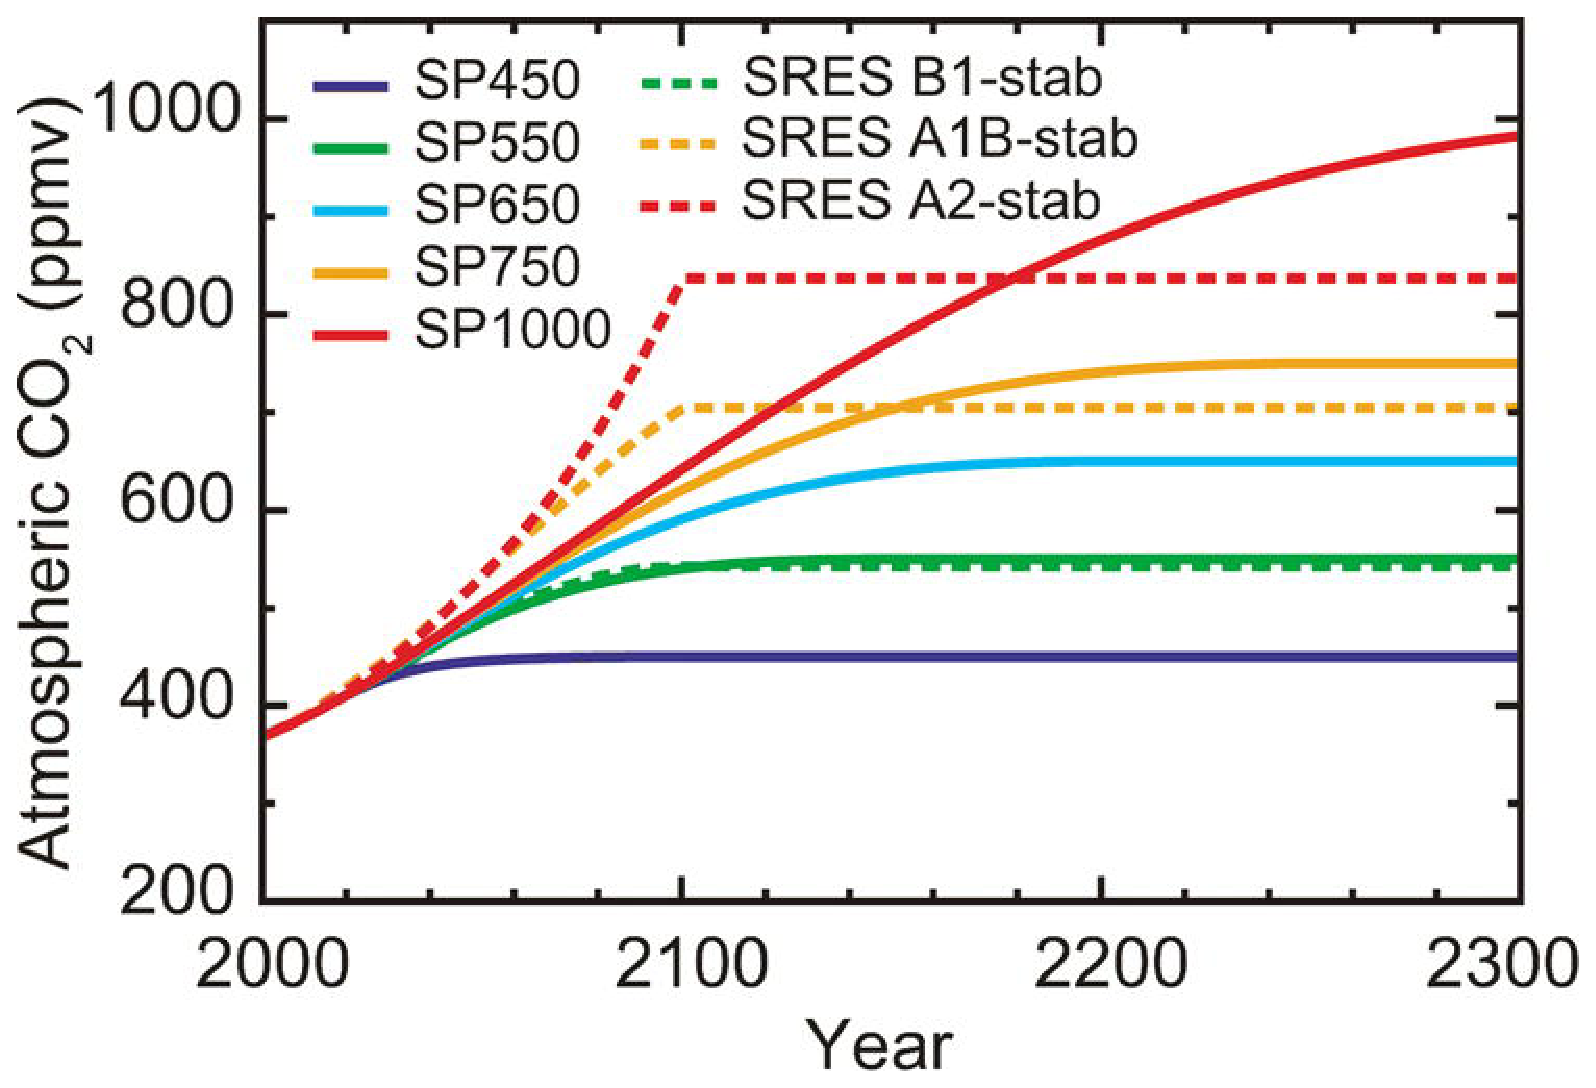
\includegraphics[width=19pc,angle=0]{./figures/figure01.eps}\\
  \caption{Enter the caption for your figure here.  Repeat as
  necessary for each of your figures. Create a figures directory and
  place all figures in that directory. Figure from Houghton et al. (2001).}\label{f1}
\end{figure}
and caption is shown above. Standard figure sizes are 
19 (one column), 27, 30, 33 (two columns), 36, and 39 picas. Authors should attempt to size their figures appropriately. At this time our press can accept only eps and TIFF figures.  Because pdfTeX does not support the use of either of these figure types authors should not attempt to build their PDF file using this driver.  The dvips driver does support the use of eps files, but not TIFF files.  Therefore, authors should use eps figure files when using this template.

\subsection{Tables}
Each table must be numbered, provided with a caption, and mentioned specifically in
the text. Each table should be in double-spaced format on a separate page, with an
explanatory caption typed above the table on the same page. All tables should be attached at
the end of the manuscript, following the figure legends. See section
11 of the Authors' Guide for more information on the proper
preparation of tables. See above for the formatting of a sample
table (Table \ref{t1}).
%%%%%%%%%%%%%%%%%%%%%%%%%%%%%%%%%%%%%%%%%%%%%%%%%%%%%%%%%%%%%%%%%%%%%
% TABLES
%%%%%%%%%%%%%%%%%%%%%%%%%%%%%%%%%%%%%%%%%%%%%%%%%%%%%%%%%%%%%%%%%%%%%
\begin{table}[t]
\caption{This is a sample table caption and table layout.  Enter as many tables as
  necessary at the end of your manuscript. Table from Lorenz (1963).}\label{t1}
\begin{center}
\begin{tabular}{ccccrrcrc}
\hline\hline
$N$ & $X$ & $Y$ & $Z$\\
\hline
 0000 & 0000 & 0010 & 0000 \\
 0005 & 0004 & 0012 & 0000 \\
 0010 & 0009 & 0020 & 0000 \\
 0015 & 0016 & 0036 & 0002 \\
 0020 & 0030 & 0066 & 0007 \\
 0025 & 0054 & 0115 & 0024 \\
\hline
\end{tabular}
\end{center}
\end{table}
%

%%%%%%%%%%%%%%%%%%%%%%%%%%%%%%%%%%%%%%%%%%%%%%%%%%%%%%%%%%%%%%%%%%%%%
% ACKNOWLEDGMENTS
%%%%%%%%%%%%%%%%%%%%%%%%%%%%%%%%%%%%%%%%%%%%%%%%%%%%%%%%%%%%%%%%%%%%%
\begin{acknowledgment}
 Keep acknowledgments (note correct spelling: no ``e'' between the ``g'' and ``m'') as brief as possible. In general, acknowledge only direct help
in writing or research. Financial support (e.g., grant numbers) for the work done, or for an
author, or for the laboratory where the work was performed is best acknowledged here rather
than as footnotes to the title or to an author's name. Contribution numbers (if the work has
been published by the author's institution or organization) should be included on the title
page, not in the acknowledgments.
\end{acknowledgment}

%%%%%%%%%%%%%%%%%%%%%%%%%%%%%%%%%%%%%%%%%%%%%%%%%%%%%%%%%%%%%%%%%%%%%
% APPENDICES
%%%%%%%%%%%%%%%%%%%%%%%%%%%%%%%%%%%%%%%%%%%%%%%%%%%%%%%%%%%%%%%%%%%%%
\ifthenelse{\boolean{dc}}
{}
{\clearpage}
\begin{appendix}[A]% Use \begin{appendix} and not \begin{appendix}[A] for only one appendix.
\section*{\begin{center}Appendix Title Is Entered Here\end{center}}
\subsection*{Appendix section}
The AMS template allows authors to format an unlimited number of appendixes.
To format a single appendix, use the $\backslash$appendix command with no additional argument. Otherwise, add the appropriate one-letter argument to the $\backslash$appendix command (e.g. $\backslash$appendix[A], $\backslash$appendix[B], $\backslash$appendix[C], etc.) corresponding to the appropriate appendix. The title of the appendix can formatted using the $\backslash$section* command as shown above (which also provides code for centering). The $\backslash$subsection, $\backslash$subsubection, and $\backslash$paragraph commands are used to create sections within the appendix. Equations are automatically numbered appropriately for each appendix. Here is an example of the first equation in appendix A, automatically labeled (\ref{eq:1}),
\begin{equation} \label{eq:1}
x=\frac{2b\pm\sqrt{b^{2}-4ac}}{2c}.
\end{equation}
\end{appendix}

\ifthenelse{\boolean{dc}}
{}
{\clearpage}
\begin{appendix}[B]
\section*{\begin{center}File structure of the AMS \LaTeX\ Package\end{center}}
\subsection*{AMS \LaTeX\ files}
You will be provided with a tarred, zipped \LaTeX\ package containing
eleven files: amspaper.tex, blank\_template.tex, ametsoc.sty, ametsoc2col.sty, amspaper.pdf, amspaper2col.pdf, figure01.eps,
AMS\_references.pdf, ametsoc.bst, database.bib, and references.bib.  Two subdirectories will be created
when you untar the package: figures and bibliography.  The figures
directory will contain the sample figure file figure01.eps.  This
directory should be used to store all your figure files.  The
bibliography directory will contain the sample bibliography files
database.bib and references.bib. You should alter references.bib with your own
bibliography information.  Refer to the AMS\_references.pdf file included in this package for information on how to properly populate the references.bib file. The files ametsoc.sty and ametsoc2col.sty are the two style files.  The file ametsoc.sty generates a PDF that follows all AMS guidelines for submission and peer review.  The file ametsoc2col.sty can be used to generate a PDF that closely follows the layout of an AMS journal page, including single spacing and two columns.  This journal style PDF is only for the author's personal use, and any papers submitted in this style will not be accepted.  Always use the ametsoc.sty when generating a PDF for submission to the AMS. The file ametsoc.bst is the bibliography style file. The file amspaper.tex contains the \LaTeX\ code for this sample file.   The resulting PDF can be seen in either amspaper.pdf or amspaper2col.pdf, depending on the which style file is used. The file blank\_template.tex provides
a basic blank template with some section headings for authors to more
easily enter their manuscript into.

Questions and feedback concerning the use of the AMS \LaTeX\ files should
be directed to latex@ametsoc.org.
\end{appendix}

\ifthenelse{\boolean{dc}}
{}
{\clearpage}
\begin{appendix}[C]
\section*{\begin{center}How to Compile the \LaTeX\ Files and Create a PDF\end{center}}
\subsection{Compilation}
There are a variety of different methods and programs that will create a final PDF from your \LaTeX\ document.  Here, the basic commands for one method of creating a final PDF are presented. You can compile your \LaTeX\ files and build the dvi file with the
following commands on a Linux-/Unix-based system:
%
%Use "enumeration" lists for numbered lists, which must use lower case roman numerals.
\begin{enumerate} 
\item latex filename.tex (e.g., latex amspaper.tex)
\item bibtex filename (e.g., bibtex amspaper).  Note that the .tex
  extension is not included in the filename
\item latex filename.tex (e.g., latex amspaper.tex)
\item latex filename.tex (e.g., latex amspaper.tex).  This command is
  repeated twice to clean up any reference dependencies.
\end{enumerate}
This will create a dvi file (e.g., amspaper.dvi).  You can view the dvi
file using a dvi file viewer, such as xdvi, kdvi, or some similar
program.  Your PDF will be created from the dvi file, so do not delete
this file.

\subsection{Creating the PDF}
The final PDF can be created from the dvi file using the following
two commands on a Linux-/Unix-based system:
\begin{itemize} % Use "itemize" lists for unnumbered lists, but bullets are not used.
\item[]{dvips filename.dvi -o filename.ps (e.g., dvips amspaper.dvi -o
  amspaper.ps), which converts the dvi file to a postscript file that
  will be converted to the final PDF; and}
\item[]{ps2pdf14 filename.ps (e.g., ps2pdf14 amspaper.ps), which creates
  the final PDF file (amspaper.pdf).  The ``14'' at the end of the ps2pdf14 command will
  generate a PDF compatible with Acrobat Reader, version 5 and later.
  It may be replaced with ps2pdf13 or ps2pdf, which will generate PDFs
  compatible with Acrobat Reader, version 4 or 3 and later,
  respectively.}
\end{itemize}
\subsection{Other software}
There is a variety of software that can be used to edit .tex files and build a PDF.  The AMS does not support \LaTeX\/-related WYSIWYG software, such as Scientific Workplace, or WYSIWYM software, such as LyX.  \TeX\ Live (available online at \url{http://www.tug.org/texlive/}) is recommended for users needing an up-to-date \LaTeX\ distribution with software that includes an editor and the ability to automatically generate a PDF.
\end{appendix}

%%%%%%%%%%%%%%%%%%%%%%%%%%%%%%%%%%%%%%%%%%%%%%%%%%%%%%%%%%%%%%%%%%%%%
% REFERENCES
%%%%%%%%%%%%%%%%%%%%%%%%%%%%%%%%%%%%%%%%%%%%%%%%%%%%%%%%%%%%%%%%%%%%%
% Create a bibliography directory and place your .bib file there.
\ifthenelse{\boolean{dc}}
{}
{\clearpage}
\bibliographystyle{ametsoc}
\bibliography{./bibliography/references}

\end{document}
%%%%%%%%%%%%%%%%%%%%%%%%%%%%%%%%%%%%%%%%%%%%%%%%%%%%%%%%%%%%%%%%%%%%%
% END OF TEMPLATE
%%%%%%%%%%%%%%%%%%%%%%%%%%%%%%%%%%%%%%%%%%%%%%%%%%%%%%%%%%%%%%%%%%%%%